\documentclass{report}
\usepackage[utf8]{inputenc}
\usepackage{graphicx}
\usepackage{verbatim}
\usepackage{circuitikz}
\usepackage{siunitx}
\usepackage{pgfplots}

\title{Vienkāršu elektrisku shēmu modelēšana}
\author{Deniss Tiščenko }
\date{Marts 2019}

\begin{document}

\maketitle



\chapter{Teorētiskā daļa}

\section{Ķēdes aprēķins}

Formulas:
$U_{R_1}=V_1*R_1/(R_1+R_2)$
\\
$U_{R_2}=V_1*R_2/(R_1+R_2)$
\\
\\
Shēmu zīmējot, izmantoju ‘pgfplots’ paku \cite{gramata1}


\begin{center}
\begin{circuitikz}[american voltages]
\draw (0,2) to[V=\SI{34.3}{\volt}]
(0,0) -- (4,0)
to[R, l=$R_2$,a=\SI{4}{\ohm}]
(4,2) -- (3,2)
to[R, l=$R_1$,a=\SI{5}{\ohm}]
(1,2) -- (0,2);
\end{circuitikz}
\end{center}


\begin{table}[h!]
\centering
\begin{tabular}{ | c | c | } 
\hline
$R_1$ & 5 \\ 
\hline
$R_2$ & 4 \\ 
\hline
$V_1$ & 34,3 \\ 
\hline
$U_{R_2}$ & 19,06 \\ 
\hline
$U_{R_1}$ & 15,24 \\ 
\hline
\end{tabular}
\caption{Tabula ar datiem \cite{gramata2}}
\label{i:example}
\end{table}


\begin{tikzpicture}
\begin{axis}[
    axis lines = left,
    xlabel = $R_2$,
    ylabel = $U_{R_2}$,
]
\addplot [
    domain=0:100,
    color=blue,
]
{34.3*x/(5+x)};
\end{axis}
\end{tikzpicture}



\chapter{Praktiskā daļa}

\section{Darbs ar GEDA programmām}

\subsection{darbs ar gschem}

\verbatiminput{02.sch}


\subsection{darbs ar gnetlist}

\subsection{darbs ar ngspice}

\begin{figure}[!tb]
\rotatebox{-90}{\includegraphics[trim= 190 300 300 300,clip,width=10cm]{01.ps}}
\caption{GEDA izveidota shēma}
\label{i:example}
\end{figure}


\section{Darbs ar QUCS programmām}

\subsection{Principāla shēma un līdzstrāvas simulācijas (DC simulation) grafiks}

\begin{figure}[!tb]
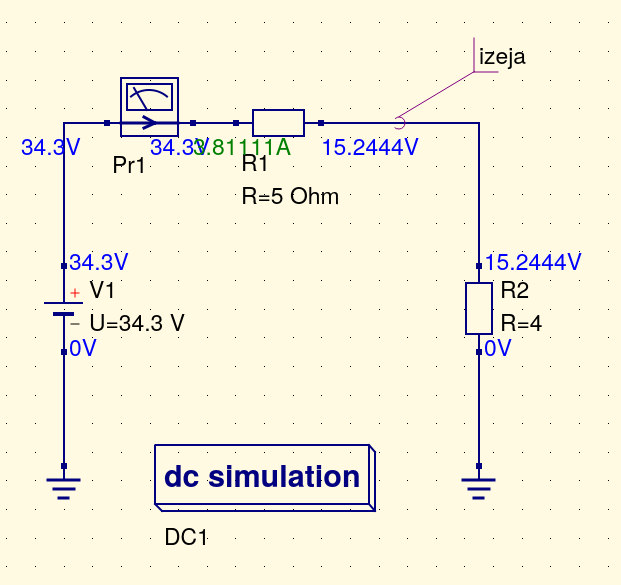
\includegraphics[width=15cm]{shema.png}
\caption{QUCS izveidota shēma un simulācija}
\label{i:example}
\end{figure}


\subsection{Sweep simulācijas grafiks un tabula}

\begin{figure}[!tb]
\rotatebox{-90}{\includegraphics[trim= 30 50 350 0,clip,width=15cm]{02.ps}}
\caption{Sweep simulācijas grafiks un tabula}
\label{i:example}
\end{figure}


\begin{thebibliography}{9}

\bibitem{gramata1}
http://texdoc.net/texmf-dist/doc/latex/circuitikz/circuitikzmanual.pdf

\bibitem{gramata2}
https://edx2.etf.rtu.lv/access/lessonbuilder/item/1882/group/1f923de4-2ba4-4a1d-8cb6-41ede04eea49/Weeks%20_e_/Week%201/P01_LV.pdf

\end{thebibliography}


\end{document}
